\chapter{Background}

%\newcommand{dltext}[1]{\centerline{\textsf{#1}\newline}}

\section{Knowledge Graphs}
There is no single agreed upon definition of \glspl{kg} \cite{bergman_2019, bonatti2019knowledge, ehrlinger2016towards}. Definitions and usages vary from specific technical proposals to more general descriptions. In this thesis we will use the more inclusive definition similar to the one proposed by Hogan et al. \cite{hogan2020knowledge}, where we view a \gls{kg} as \textit{a graph of data intended to capture the semantic connections within real world knowledge, where nodes represent relevant entities and edges represent relations between these entities}. The type of graph may vary, i.e. it may be simple, directed, etc. A graph may contain knowledge over a broad range of domains, such as Wikidata\cite{lehmann2015dbpedia}, or be limited to a specific domain, such as DBpedia\cite{fellbaum2010wordnet}. The concept of ``knowledge'' has been widely debated in epistemology, but here we will use it to mean descriptive knowledge, meaning facts that can be stated. Knowledge can be simple statements, such as ``Leo is a cat'', or quantified statements such as ``at least one cat is black''. KGs are not expressive enough for quantified statements, where ontologies or rules would be more appropriate. Additional knowledge can be inferred from KGs through inductive or deductive methods. For example from a KG containing the information that ``Leo is a cat'' and ``cats are mammals'', one can deductively infer that ``Leo is a mammal''. If all cats mentioned in the knowledge graph like to eat fish, then one can inductively infer ``cats like to eat fish''.


%For example, the knowledge that 'Amy is the daughter of Bo, and Bo is a woman' can be represented by the knowledge graph in fig 1.\todo{Add figure}
\begin{figure}
\centering
\begin{tikzpicture}
    \node[shape=circle,draw=red] (L) at (0,0) {Leo};
    \node[shape=circle,draw=black] (C) at (3,0) {Cat};
    \node[shape=circle,draw=black] (M) at (1.5,3) {Mammal};

   % \path [->] (L) edge node[left] {$IsA$} (C);
   \draw [->] (L) -- (C);
   \draw [decoration={text along path,
    text={is a},text align={center}},decorate]  (L) -- (C);
    
    \draw [->] (C) -- (M);
   \draw [decoration={text along path,
    text={subclass},text align={center}},decorate]  (M) -- (C);
    
    \draw [dotted, ->] (L) -- (M);
   \draw [decoration={text along path,
    text={is a},text align={center}},decorate]  (L) -- (M);
    
\end{tikzpicture}

\caption{Example of a knowledge graph, where the dotted line represents a relationship that can be deductively inferred.} \label{fig:KGexample}
\end{figure}

\newpage

In this thesis we will loosely follow the Resource Description Framework (RDF) standard and view KGs as sets of semantic triples. RDF is a standard for representation and exchange of graph data introduced by \gls{w3c}. Semantic triples are the data types used in the RDF data model. A triple, as the name suggests, is a tuple of three elements. It has the form ( subject, predicate, object) and can therefore represent statements about semantic data, for example "Cats are mammals", or "Ann knows Bob". These RDF statements express relationships between two resources, these resources being the subject and the object, while the predicate encapsulates the nature of the relationship. The relationship is phrased in a directional way, and so set of RDF stamements can also be viewed as a directed graph. The graph represents these triple statements, where the predicate in the triple denotes the edge going from the subject to the object, both of which are vertices.

\begin{lstlisting}[caption={Example of RDF triple set written in informal pseudocode},label={RDF_triples_example}]
<Ann> <knows> <Bob>
<Ann> <is a> <person>
<Bob> <is a> <person>
<Ann> <owns> <Leo>
<Leo> <is a> <cat>
<cat> <is a> <mammal>
<Bob> <is scared of> <Leo>
\end{lstlisting}

\begin{figure}
\centering
    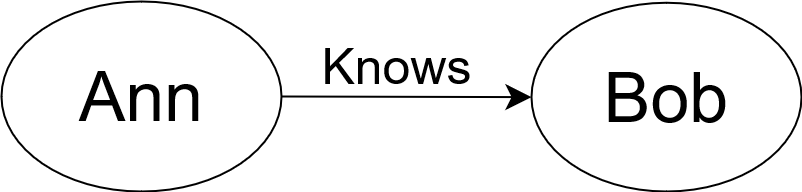
\includegraphics[scale=0.3]{figures/RDF_triple}
    \caption{TODO Informal graph of the example triples from \ref{RDF_triples_example}}
    
    \label{fig:KGexample}
\end{figure}

With this type of data organisation one can for example query for a list of all people who own cats in the dataset. 
\subsection{Open versus closed world assumption}

\section{Knowledge Graph Embeddings}
Let a KG be defined as a set of triples $\mathcal{K}={<h, r, t>}$, where $h, r, t$ respectively denote the head entity, relation and tail entity. To simplify the explanation we let the dimension of entities \emph{and} relations in the embedding space to be $d$.
Given $\mathcal{K}$ and $d$, a KG embedding seeks to represent all entities and relations in the continuous vector space of $d$ dimensions. These representations are meant to capture the semantic information in the graph. An embedding that manages this can then be used to evaluate the probability of new facts (link prediction) and identify false information in $\mathcal{K}$.




Where do the negative examples come from?: https://ieeexplore.ieee.org/stamp/stamp.jsp?tp=&arnumber=7358050
\subsection{Triple corruption}
Let $\mathcal{K}$ be KG with triples of the form $<h, r, t>$ with $r\in \mathbb{R}$ and $h, t \in \mathbb{E}$, where $\mathbb{R}$ and $\mathbb{E}$ are respectively the set of all relations and entities in $\mathcal{K}$. The set of corrupted triples $\mathcal{K'}$ is generated by taking triples from the KG and swapping the $h$ or $t$ (not both) with some other $h', t' \in \mathbb{E}$ \cite{TransE}.
\begin{equation}
   \mathcal{K'} =\{<h', r, t> |h' \in \mathbb{E} \} \cup \{<h, r , t'> | t' \in \mathbb{E}\}
\end{equation}



\textbf{Metrics}

    Ranking triples

    MR

    MRR

    Hits@n
    
    
\begin{figure}[htp]
    \centering
    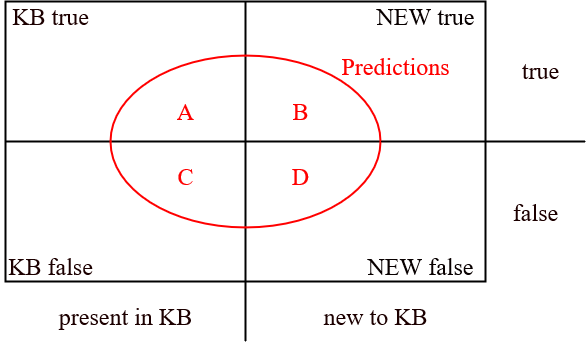
\includegraphics[width=10cm]{figures/kb_venn.png}
    \caption{KB prediction under incompleteness}
\end{figure}


\section{Rule-based machine learning}
Rule-based machine learning has as a goal to create rules that make new true predictions going beyond the data on which the rule was applied to. In contrast, other areas of machine learning focus on training a single model that can be applied to make a broad range of predictions. Conceptually the end result of rule-based machine learning is similar to a rule-based system.  Rule-based systems are often hand-crafted and require a knowledge expert to be curated, while rule-based machine learning requires no knowledge expert and rules are automatically created by the learning algorithm.

Classically, a rule is comprised of a condition and consequent, or a so-called "if-then" statement. \begin{center} \textbf{IF} \textit{'the condition is met'} \textbf{THEN} \textit{'the consequent holds'} \end{center}
The condition of the rule specifies attributes in the data on which the rule will be applied. If these attributes are present in this data, the condition is met. Once the condition for the rule is met, the attributes in the consequent should neccesarily also be met.

\begin{equation}
hasSibling(x, y) \Rightarrow hasSibling(y,x)
\label{example_rule_1}
\end{equation}
\begin{equation}
    hasSibling(x, y) \Rightarrow hasMother(x,z) \Rightarrow hasMOther(x, z)
    \label{example_rule_2}
\end{equation}
\begin{lstlisting}[caption={Simple example knowledge base},captionpos=b, label={simple_kb_example}]
<Ann> <hasMother> <Carol>
<Ann> <hasSibling> <Bob>
<Bob> <hasSibling> <Ann>
\end{lstlisting}
Consider the two rules and knowledge base given above. Under this knowledge base the antecedent of the first rule is satisfied by both triple 2 and 3. The resulting consequent of rule \ref{example_rule_1} is also present in the knowledge base. So the reflexivity of the $hasSibling$ predicate holds in this knowledge base. The antecendent of the second rule is satisfied by triples 1 and 2 in the knowledge base, but the resulting consquent would then be $hasMother(Bob, Carol)$. Since \texttt{<BoB> <hasMother> <Carol>} is not present in the knowledge base, rule \ref{example_rule_2} does not hold. If we know that this rule is reliable, we could for example extend the incomplete knowledge base with this triple.

Within rule-based machine learning there are many different approaches including learning classifier systems\cite{sigaud2007learning} and association rule mining\cite{agrawal1993mining}, the latter of which is the approach used in this thesis. Both approaches aim to create a set of rules to act as a model for a set of data. The association rule mining approach will now be explained further.


\subsection{Association Rule Mining}
Association rules \cite{agrawal1993mining} are types of "if-then" statements that describe frequent associations between items in a dataset containing \textit{transactions}. Association rule mining was originally proposed as a new method for finding relationships between sales items in stores. The idea of mining association rules over transactions has successfully been applied to many other scenarios \cite{altaf2017applications, lin2002efficient}. In the context of convenience store sales, each transaction can be thought of as a set of items that a customer has purchased. The rules are of the form $\{Sugar, Flour, Eggs\} \Rightarrow Butter$, meaning that a person who bought sugar, flour and eggs was likely to also purchase butter. The antecedent is some set of items in the dataset, while the consequent is an item often found in combination with the antecedent in the dataset.  So sugar, flour and eggs can be thought of as "associated with" butter. These original association rules are also not Horn rules over binary predicates, but is cited as a main inspiration for the AMIE approach used for experiments in this thesis.

\subsection{Significance and quality measurement}
The goal is to find formal rules that make true predictions that go beyond the explicit information in the knowledge base. For this some for of metrics are required in order to determine the suitability of a proposed rule.




Support and confidence were originally proposed as relevance and quality measurements for this type of rule mining, but as explained in \todo{PCA m8} this is not adequate when working with datasets in the form of knowledge graphs.

\[supp(\vec{B}\Rightarrow r(x, y)) :=  \# (x, y) : \exists z_1 , ...,z_m : \vec{B} \wedge r(x, y)\]

\[hc(\vec{B}\Rightarrow r(x, y)) := \frac{supp(\vec{B}\Rightarrow r(x, y)}{ \#(x', y'):r(x', y'))}\]

\[conf(\vec{B}\Rightarrow r(x, y)) := \frac{supp(\vec{B}\Rightarrow r(x, y)}{\#(x, y):\exists z_1 ,..., z_m : \vec{B}}\]

Partial completeness
\[\forall y' : r(x, y') \in KBtrue \cup NEWtrue \Rightarrow r(x, y') \in KBtrue\]

\[pcaconf(\vec{B}\Rightarrow r(x, y)) := \frac{supp(\vec{B}\Rightarrow r(x, y)}{\#(x, y):\exists z_1 ,..., z_m, y' : \vec{B} \wedge r(x, y')}\]


\subsection{AMIE+}

\iffalse 
\section{Web Ontology Language}
A widely used formal language for expressing ontologies is the \gls{owl}. In OWL "Daughters are female" could be formally expressed as:

\centerline{\textsf{SubClassOf(Daughter Female)}}
Information expressed in OWL can be used to draw new conclusions. For example if we know that an individual \emph{Amy} is a daughter, then we can makes the same conclusions as earlier about Amy being female. In OWL, the fact that Amy is in the class of females can be expressed as:

\centerline{\textsf{ClassAssertion(Female amy)}}
The task of reaching such conclusions is called reasoning and the type of conclusions that can be drawn is specified by the \gls{w3c}. It specifies the \emph{semantics} of OWL, but does not present algorithms for how to derive inferences in practice. Sound and complete reasoning in OWL is of high complexity \cite{Krotzsch2012}. Therefore, when the standard was updated to OWL 2 in 2009, it introduced restricted sublanguages to address this problem. These sublanguages restrict expressivity in order to simplify the reasoning task. One of these languages is OWL 2 QL, which is based on a \gls{dl} language called DL-Lite. OWL 2 QL is intended as a language to enable easier queries to databases. The ontology language we will use is DL-Lite$_{\mathcal{R}, horn}^{\exists}$, which is a member of the DL-Lite family.



\section{Description Logics}
\gls{dls} are a family of languages used in knowledge representation and reasoning. They are generally less expressive than \gls{fol}, but more expressive than \gls{pl}. The name \textit{description logic} represents two central aspects to this language group: \emph{description}, formal expression of knowledge, and  \emph{logic}, for it's logic-based semantics. DLs are used to represent domain knowledge in a well-structured and easily interpretable way. Domain knowledge is separated into two components in DL, a \emph{terminological} part, called a TBox, and an \emph{assertional} part, called an ABox. The TBox represents knowledge about the structure of the domain, while the ABox has knowledge about specific instances. For example the fact that \emph{cats are  mammals} would be a TBox statement, while \emph{Leo is a cat} would be an ABox statement, as here we are making an assertion about the individual Leo. The combination of a TBox and an ABox is called a \emph{knowledge base} (KB).
As the semantics of DLs are logic-based it is clear when a statement is \emph{entailed} by a KB. For instance the two examples given above entail that Leo is a mammal. More importantly, this reasoning task can be automated in a DL KB. Reasoning tasks are performed with respect to the entire KB, which gives this language great power, but also comes with a computational cost. Therefore an important area of research has been to find DLs that strike a balance between expressiveness and the computational complexity of reasoning.


The two main criteria for a reasoner is that it is decidable and tractable (always correctly completed in a time that is polynomial with respect to the size of the KB). The more operators one allows in a logic the more complicated the TBox becomes, and usually the complexity for reasoning in the language increases. See \href{http://www.cs.man.ac.uk/~ezolin/dl/}{\textbf{Complexity of reasoning in Description Logics}} for an interactive look at the complexity of different DLs \cite{zolin_2013}.

\section{The Resource Description Framework}

The Resource Description Framework (RDF) is a standard for representation and exchange of graph data introduced by \gls{w3c}. Semantic triples are the data types used in the RDF data model. A triple, as the name suggests, is a tuple of three elements. It has the form ( subject, predicate, object) and can therefore represent statements about semantic data, for example "Cats are mammals", or "Ann knows Bob". These RDF statements express relationships between two resources, these resources being the subject and the object, while the predicate encapsulates the nature of the relationship. The relationship is phrased in a directional way, and so set of RDF stamements can also be viewed as a directed graph. The graph represents these triple statements, where the predicate in the triple denotes the edge going from the subject to the object, both of which are vertices.

\begin{lstlisting}[caption={Example of RDF triple set written in informal pseudocode},label={RDF_triples_example}]
<Ann> <knows> <Bob>
<Ann> <is a> <person>
<Bob> <is a> <person>
<Ann> <owns> <Leo>
<Leo> <is a> <cat>
<cat> <is a> <mammal>
<Bob> <is scared of> <Leo>
\end{lstlisting}

\begin{figure}
\centering
    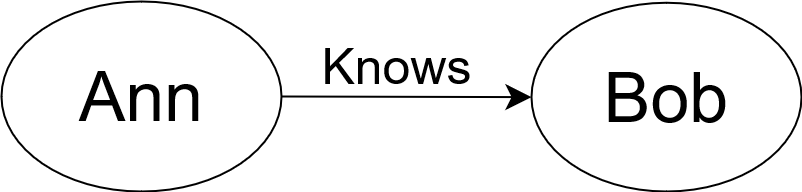
\includegraphics[scale=0.3]{figures/RDF_triple}
    \caption{TODO Informal graph of the example triples from \ref{RDF_triples_example}}
    
    \label{fig:KGexample}
\end{figure}

With this type of data organisation one can for example query for a list of all people who own cats in the dataset.

\subsection{Resource Description Framework Schema}
RDF provides the abstract model for how to organize the data and sets standards for how data points relate to eachother and real-world entities. The RDF Schema (RDFS), on the other hand, is a \emph{vocabulary} in RDF that explains how nodes of a graph relate.

\section{Semantic Triples in Description Logics}
Semantic triples are 
\fi
